\clearpage
\section{Auswertung}

\subsection{Lipide}

Untersucht wurden im Folgenden die Peaks von [PC(32:0)+H]$^+$ bei \SI{734.562}{} und [PC(34:1)+H]$^+$ bei \SI{760,578}{}.
In \cref{fig_broken} sind zwei Massenspektren dargestellt, die sich insofern von den meisten aufgenommenen Spektren unterscheiden, als dass ein starkes Untergrundsignal vorliegt, welches entweder auf Verunreinigungen in der Probe zurückzuführen ist.
Auch denkbar ist, dass bei sehr geringer Analytkonzentration mehr Untergrund ionisiert und gemessen wird.
In \cref{fig_very_broken} sind dabei die zu untersuchenden Peaks nicht mehr zu erkennen, weshalb dieses und ein weiteres Spektrum dieser Art nicht verwendet werden können.
Im Gegensatz dazu ist in \cref{fig_fine_broken} das Signal noch deutlich zu erkennen, weshalb die sechs Spektren dieser Art ausgewertet werden.

\begin{figure}[!ht]
    \centering
    \begin{subfigure}{0.495\textwidth}
        \centering
        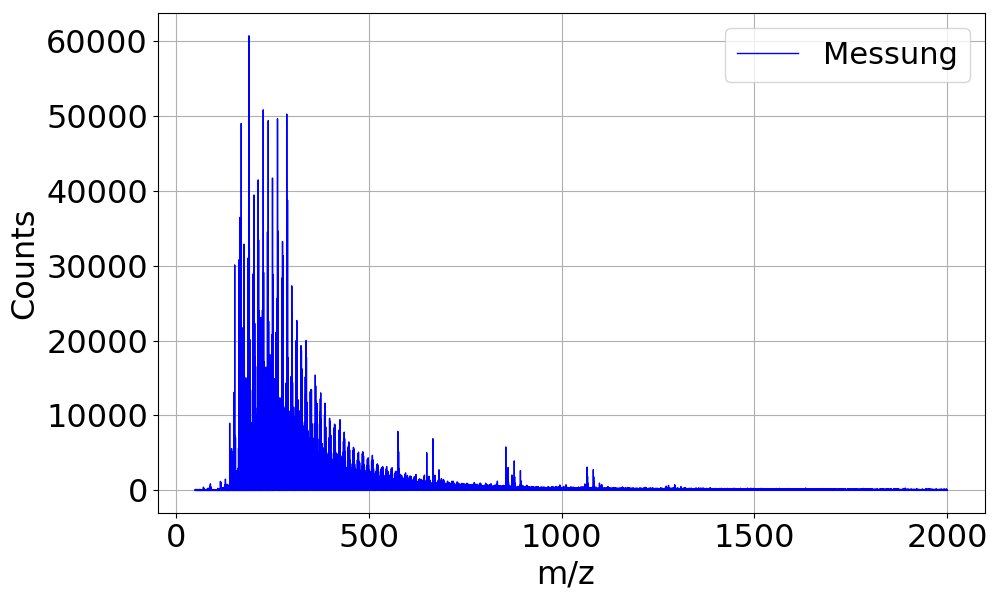
\includegraphics[width=1.0\textwidth]{img/b11_S_broken}
        \caption{CHCA $10^{-6}$ \si{\mole \per \liter}}
        \label{fig_very_broken}
    \end{subfigure}
    \begin{subfigure}{0.495\textwidth}
        \centering
        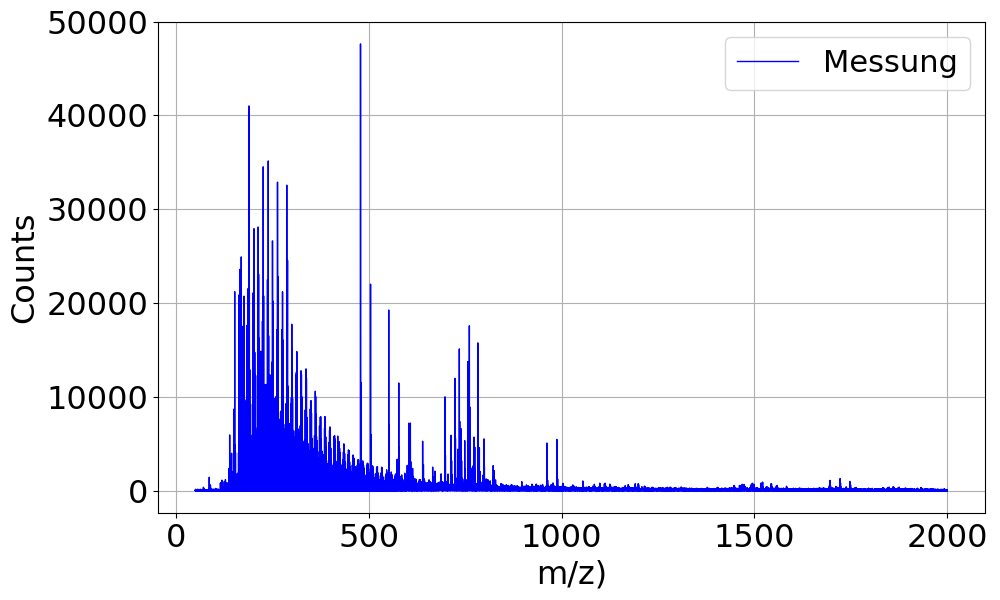
\includegraphics[width=1.0\textwidth]{img/C11_S_broken_but_fine}
        \caption{CHCA $10^{-5}$ \si{\mole \per \liter}}
        \label{fig_fine_broken}
    \end{subfigure}
    \caption{Zwei Massenspektren mit großem Untergrundsignal bei Matrix CHCA und unterschiedlichen Analytkonzentrationen. Beide im S-Modus.}
    \label{fig_broken}
\end{figure}

Zur Auswertung der Spektren wird für jedes Spektrum und beide untersuchte Peaks ein lokaler Gauß-Fit durchgeführt, von denen einer in \cref{fig_gaussfit} abgebildet ist.
Aus den Fit-Parametern werden Signalstärke, Peakposition (Masse-zu-Ladung-Verhältnis), Halbwertsbreite und ein als lokal konstant angenommener Untergrund entnommen.

\begin{figure}[!ht]
    \centering
    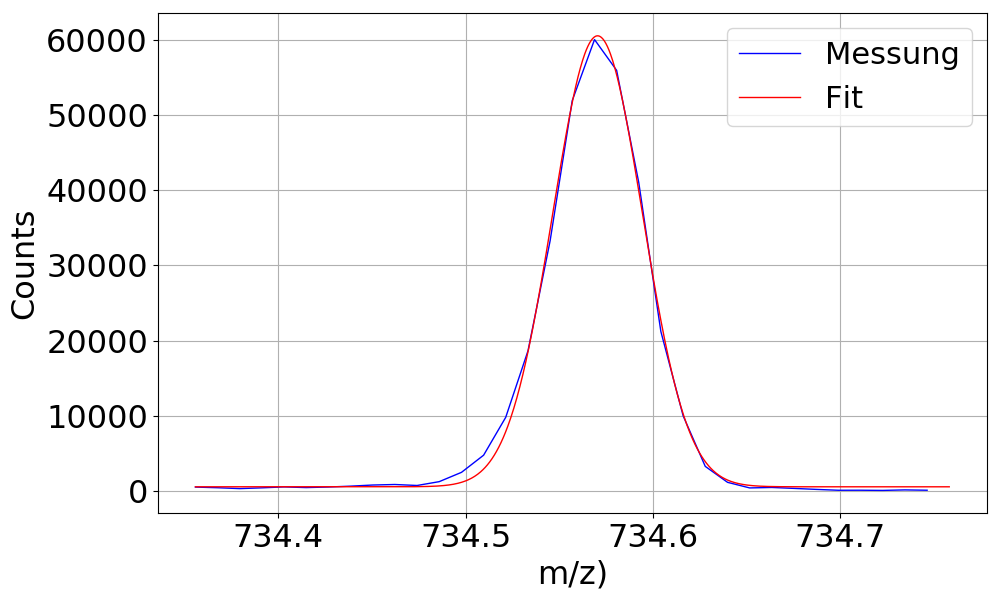
\includegraphics[width=0.6\textwidth]{img/a04_S_gaussfit}
    \caption{Gauß-Fit bei Matrix DHB und einer Analytkonzentration von $10^{-7}$ \si{\mole \per \liter}.}
    \label{fig_gaussfit}
\end{figure}

Sofern mindestens zwei Spektren zur Verfügung stehen, wird für die Ergebnisse ein Mittelwert und die Standardunsicherheit bestimmt und im Folgenden als Unsicherheit verwendet.
Eine Tabelle mit den Ergebnissen aller Fits bei allen Spektren findet sich in \cref{sec:anhang}.

Um die Massenauflösung $R=\frac{m}{\Delta m}$ zu bestimmen und den HR-Modus mit dem S-Modus zu vergleichen, wird jeweils das Masse-zu-Ladung-Verhältnis durch die Halbwertsbreite geteilt.
Die Ergebnisse sind in \cref{tab:HR-S-vgl} dargestellt.
Es ist deutlich zu erkennen, dass die Massenauflösung im HR-Modus wie erwartet deutlich größer ist.
Außerdem ist sie bei Verwendung von  DHB als Matrix im S-Modus etwas größer als bei CHCA und im HR-Modus etwas kleiner.
Es ist auch sichtbar, dass die Standardunsicherheit im S-Modus um etwa eine Größenordnung geringer ist, also die Massengenauigkeit höher ist.

\begin{table}[H]
	\centering
	\caption{Ergebnisse aus den Fits ausgewählter Peaks in den Massenspektren nach Matrix und Modus des Flugzeitspektrometers. Die Verdünnungsstufe beträgt $10^{-4}$ \si{\mole \per \liter}.}
	   \begin{tabular}{c | c | c | c }
      Modus & Matrix & $m/z$ & Massenauflösung $R$ \\ \hline
      S & CHCA & \SI{734,56818 \pm 0,00018}{} & \SI{12717 \pm 57}{} \\
        &      & \SI{760,58348 \pm 0,00020}{} & \SI{12788 \pm 306}{} \\
        & DHB  & \SI{734,56951 \pm 0,00011}{} & \SI{14645 \pm 450}{} \\
        &      & \SI{760,58491 \pm 0,00022}{} & \SI{14634 \pm 540}{} \\
      HR& CHCA & \SI{734,5653  \pm 0,0014}{}  & \SI{39841 \pm 657}{} \\
        &      & \SI{760,5811  \pm 0,0010}{}  & \SI{38488 \pm 2688}{} \\
        & DHB  & \SI{734,5643  \pm 0,0018}{}  & \SI{36596 \pm 2531}{} \\
        &      & \SI{760,5801  \pm 0,0011}{}  & \SI{36686 \pm 1287}{} \\
	\end{tabular}
	\label{tab:HR-S-vgl}
\end{table}

Nun soll noch Massengenauigkeit und Massenrichtigkeit bei verschiedenen Verdünnungsstufen verglichen werden.
Hierfür wird der Sensitivity-Modus verwendet, weil hier ein besseres Signal-Rausch-Verhältnis zu erwarten ist und die Massenauflösung auch hier groß genug ist, um die betrachteten Peaks eindeutig voneinander trennen zu können.
Die Massengenauigkeit wird wie oben über die Standardunsicherheit bestimmt.
Wenn nur ein Spektrum zur Verfügung steht, wird die Unsicherheit, die sich aus dem Fit ergibt, verwendet.
In diesem Fall werden die Daten mit einem $*$ gekennzeichnet.
Für die Massenrichtigkeit wird die Differenz zwischen Mittelwert der gemessenen Masse-zu-Ladung-Verhältnisse und dem erwarteten exakten Masse-zu-Ladung-Verhältnis des jeweiligen Moleküls gebildet.
Da für die exakte Masse des Moleküls Werte mit drei Nachkommastellen angegeben wurden, ergibt sich für die Massenrichtigkeit eine zusätzliche digitale Unsicherheit von $\approxeq \SI{0.0003}{}$.
Außerdem wird das Signal-Rausch-Verhältnis bestimmt, indem die Höhe des gefitteten Gauß-Peaks durch die Größe des lokalen konstanten Untergrunds geteilt wird.
Wie in \cref{fig_gaussfit} zu erkennen ist, ist die Annahme eines konstanten Untergrund in guter Näherung gerechtfertigt und da die betrachteten Peaks deutlich voneinander getrennt sind, ist auch nicht zu befürchten, dass ein Teil der Höhe der Peaks auf eine Überlappung mit anderen Peaks zurückzuführen ist.
In einigen Fällen treten jedoch deutlich kleinere Peaks im Bereich des lokalen Fits auf, die mittels dieser Methode nur als Anteil am konstanten Untergrund gewertet werden.
Auch hier wird, wenn möglich, ein Mittelwert verwendet und die Standardunsicherheit angegeben.
Die Ergebnisse sind in \cref{tab:verduennungen} aufgeführt.

\begin{table}[H]
	\centering
	\caption{Massengenauigkeit, -richtigkeit und Signal-Rausch-Verhältnis (SRV) aus den Fits ausgewählter Peaks in den Massenspektren nach Matrix und Verdünnungsstufe. Die Spektren wurden im Sensitivity-Modus aufgenommen. $*$ markiert, wenn für die Berechnung nur ein Spektrum zur Verfügung steht, weshalb hier der Fehler aus dem Fit verwendet wird. Verdünnung in \si{\mole \per \liter}}
	   \begin{tabular}{c | c | c | c  | c | c}
      Verd. & Matrix & $m/z$ & Massenrichtigkeit & SRV \\ \hline
      $10^{-4}$ & CHCA & \SI{734,56818 \pm 0,00018}{} & \SI{0,00619 \pm 0,00034}{} & \SI{110,3 \pm 3,4}{}\\
                &      & \SI{760,58348 \pm 0,00020}{} & \SI{0,00548 \pm 0,00035}{} & \SI{133 \pm 18}{}\\
                & DHB  & \SI{734,56951 \pm 0,00011}{} & \SI{0,00751 \pm 0,00031}{} & \SI{136,8 \pm 9,5}{}\\
                &      & \SI{760,58491 \pm 0,00022}{} & \SI{0,00691 \pm 0,00037}{} & \SI{142,6 \pm 3,5}{}\\
      $10^{-5}$ & CHCA & \SI{734,57021 \pm 0,00023}{} $*$ & \SI{0,00821 \pm 0,00037}{} & \SI{65 \pm 11}{}\\
                &      & \SI{760,58573 \pm 0,00025}{} $*$ & \SI{0,00773 \pm 0,00038}{} & \SI{74 \pm 12}{} \\
                &  DHB & \SI{734,57025 \pm 0,00024}{} $*$ & \SI{0,00825 \pm 0,00038}{} & \SI{81 \pm 16}{}\\
                &      & \SI{760,58590 \pm 0,00022}{} $*$ & \SI{0,00790 \pm 0,00036}{} & \SI{108 \pm 33}{}\\
      $10^{-6}$ & DHB  & \SI{734,56906 \pm 0,0007 }{} $*$ & \SI{0,00706 \pm 0,00076}{} & \SI{17 \pm 2}{}\\
                &      & \SI{760,58529 \pm 0,0006 }{} $*$ & \SI{0,00729 \pm 0,00067}{} & \SI{21 \pm 3}{}\\
      $10^{-7}$ & DHB  & \SI{734,57022 \pm 0,00030}{} & \SI{0,00822 \pm 0,00042}{} & \SI{93 \pm 11}{}\\
                &      & \SI{760,58569 \pm 0,00027}{} & \SI{0,00769 \pm 0,00039}{} & \SI{71 \pm 27}{}\\
	\end{tabular}
	\label{tab:verduennungen}
\end{table}

Für den Vergleich der Verdünnungsstufen soll sich auf DHB konzentriert werden, da hier mehr Spektren aufgenommen wurden.
Die Massengenauigkeit scheint mit sinkender Verdünnung schlechter zu werden (der Zahlenwert der Standardunsicherheit nimmt zu).
Dies kann jedoch aufgrund mangelnder Spektren nur an zwei Verdünnungsstufen festgemacht werden.

Bei der Massenrichtigkeit ist kein signifikanter Trend zu erkennen.
Dies ist nicht verwunderlich, da die Massenrichtigkeit vor allem von der Kalibrierung abhängt, welche für alle aufgenommenen Spektren gleich ist.

Anhand der Daten für die Verdünnungsstufen $10^{-4}$, $10^{-5}$ und $10^{-6}$ \si{\mole \per \liter} lässt sich feststellen, dass das Signal-Rausch-Verhältnis mit der Analytkonzentration deutlich abnimmt.
Bei DHB wurde bei der Verdünnungsstufe von $10^{-7}$ \si{\mole \per \liter} vermutlich ein Fehler in der Präparation gemacht, da hier der Trend gebrochen wird und das Signal-Rausch-Verhältnis wieder deutlich ansteigt
\par

Anhand der vorherigen Ergebnisse wird als Spektrum mit optimalen Bedingungen für ein Übersichtsbild DHB bei einer Verdünnungsstufe von $10^{-4}$ \si{\mole \per \liter} im Sensitivity-Modus gewählt.
In \cref{fig_gesamtspekt} ist dieses Spektrum dargestellt und der rote Ausschnitt ist in \cref{fig:teilspekt} vergrößert dargestellt.
Dort wurden die Peaks den verschiedenen Lipidspezies zugeordnet.

\begin{figure}[!ht]
    \centering
    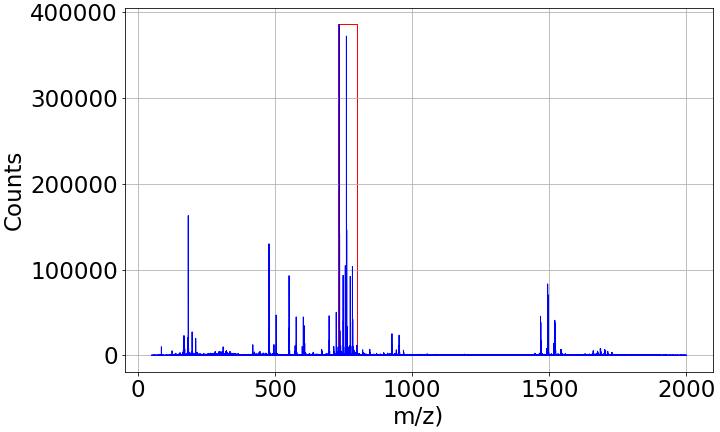
\includegraphics[width=1\textwidth]{img/overview-D02_Oben_S}
    \caption{Gemessenes Gesamtspektrum bei Matrix DHB, Verdünnungsstufe $10^{-4}$ \si{\mole \per \liter} und im Sensitivity-Modus.}
    \label{fig_gesamtspekt}
\end{figure}

\begin{figure}[!ht]
    \centering
    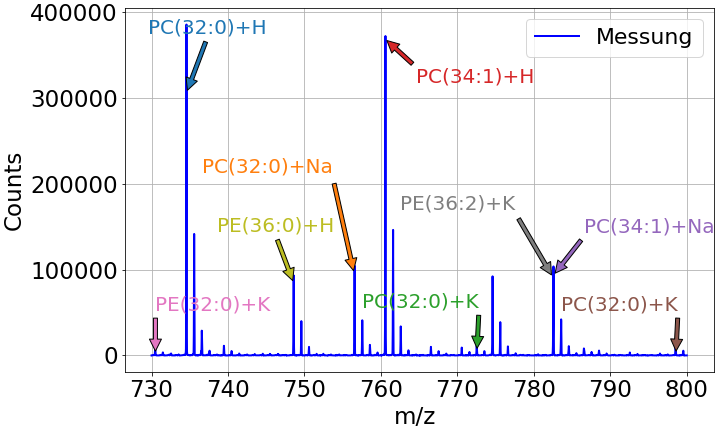
\includegraphics[width=1\textwidth]{img/overview_zoom-D02_Oben_S}
    \caption{Annotierter Ausschnitt aus dem gemessenen Spektrum bei Matrix DHB, Verdünnungsstufe $10^{-4}$ \si{\mole \per \liter} und im Sensitivity-Modus.}
    \label{fig:teilspekt}
\end{figure}


\subsection{Imaging}

Es ist möglich, das Bild über die gemessene Gesamtionenzahl (TIC, Total Ion Count) des im jeweiligen Pixel zu normieren. %ich denke, dass Gesamtzahl aller Ionen im Pixel und nicht des einzelnen Ions im Bild gemeint ist.
Dies verursacht hier nur eine geringfügige Änderung des Bildes, erlaubt aber zu erkennen, falls der Probenschnitt nicht gerade geschnitten ist, da in diesem Fall manche Pixel weniger Ionenausbeute hätten.

In \cref{fig:hirn1} ist das Imaging-Bild bei Auswahl von Ionen mit Masse-zu-Ladung-Verhältnis von \SI{772.546}{} dargestellt.
Anhand der Referenzbilder von \emph{reference atlas viewers} \cite{mouse-brain-map} lässt sich dies etwa Coronal-Ebene 118 (Bregma \SI{-6,455}{mm}) zuordnen.
Das Referenzbild ist in \cref{fig:hirn-ref} abgebildet.
Dabei fällt auf, dass im oberen Bereich des Bildes die Probe leicht beschädigt ist.

\begin{figure}[!ht]
    \centering
    \begin{subfigure}{0.65\textwidth}
        \centering
        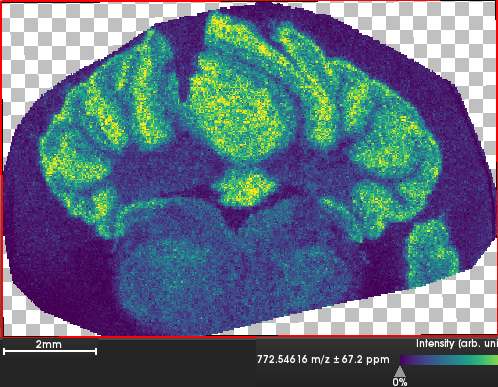
\includegraphics[width=1\textwidth]{raw/hirn/Hirn772_crop}
        \caption{MALDI-Aufnahme}
        \label{fig:hirn1}
    \end{subfigure}
    \begin{subfigure}{0.65\textwidth}
        \centering
        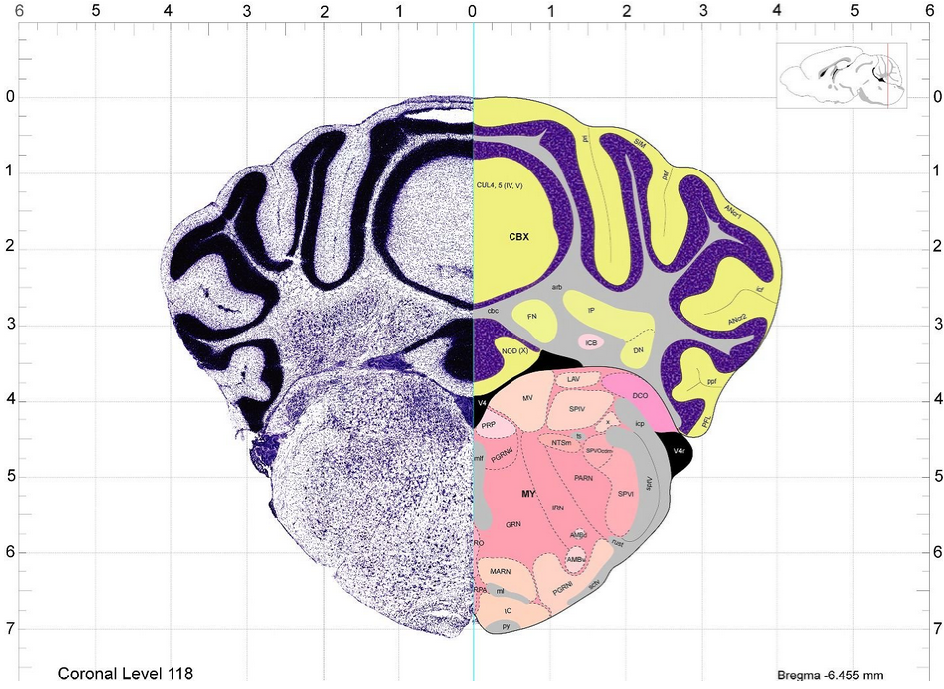
\includegraphics[width=1\textwidth]{img/coronal_ref}
        \caption{Referenzbild}
        \label{fig:hirn-ref}
    \end{subfigure}
    \caption{(a) MALDI-Imaging-Aufnahme eines Coronal-Schnittes eines Mäusehirns. (b) Zugeordnetes Referenzbild des verwendeten Coronal-Schnittes. \cite{mouse-brain-map}}
    \label{fig:hirn-vgl}
\end{figure}

Nun werden mithilfe des \emph{interactive atlas viewers} die bei der jeweiligen Ionenauswahl sichtbaren Bereiche identifiziert und in \cref{fig:hirn-ann} beschriftet dargestellt.
Dabei wurden die Ionen mit $m/z$ von \SI{838.60667}{} und \SI{872.52693} ausgewählt und in unterschiedlichen Farben dargestellt, um möglichst viel Kontrast zwischen unterschiedlichen Strukturen zu erreichen.

Die gelben astförmigen Strukturen im oberen Bereich können leicht als Arbor Vitae identifiziert werden, welcher umgeben von der in Rot sichtbaren Kleinhirnrinde (cerebellar cortex) ist.
Im unteren Bereich ist in Gelb die Medulla zu erkennen, während der  vierte Hirnventrikel in der Mitte beide ausgewählte Ionen nur in geringer Menge emittiert, also schwarz erscheint. %Groß/klein schwierig, weil engliches Latein
Die dunkle Schicht zwischen Kleinhirnrinde und Arbor Vitae ist die Körnerschicht.

\begin{figure}[!ht]
    \centering
    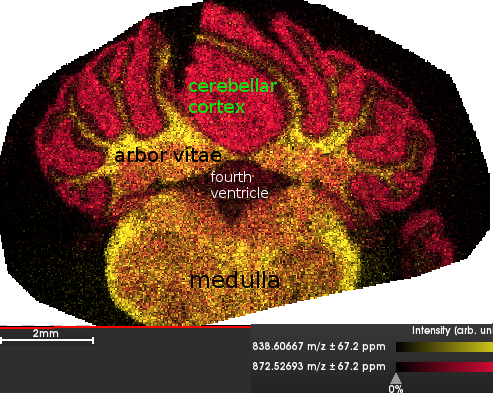
\includegraphics[width=1\textwidth]{raw/hirn/Hirn872-838_ann}
    \caption{Annotierte MALDI-Imaging-Aufnahme eines Coronal-Schnittes eines Mäusehirns.}
    \label{fig:hirn-ann}
\end{figure}
